\documentclass{beamer}

\usepackage[utf8]{inputenc}
\usepackage{graphicx}

\title{Case Study 2-Group 4}
\author{Frances Hung, Yunran Chen, Keru Wu}
\institute{Department of Statistical Science, Duke University}
\date{01/30/2019}

\begin{document}

\frame{\titlepage}



%%%%%%%%%% Section1: Introduction %%%%%%%%%%%


\begin{frame}
\frametitle{Introduction}

\begin{itemize}
\item Data:  2019 Airbnb listings in NYC, 48895 observations.
  
\item Goal: Identify discernible and interesting patterns among the listings in NYC.

\end{itemize}

\end{frame}






%%%%%%%%%% Section2: Materials & Methods %%%%%%%%%%%

\begin{frame}
\frametitle{Data Preprocessing}
\begin{itemize}
\item Delete id, host\_name and last\_review.
\item Delete 11 listings with price 0.
\item Missing data: 10052 in reviews\_per\_month, impute with 0.
\item Categorize minimum\_nights to 5 groups: 1-2, 3-6, 7-13, 14-20, 21-27, 28+ days. 
\item Transformation: log(price), log(1+reviews\_per\_month). 
\end{itemize}

\end{frame}



\begin{frame}
    \frametitle{EDA-borough}
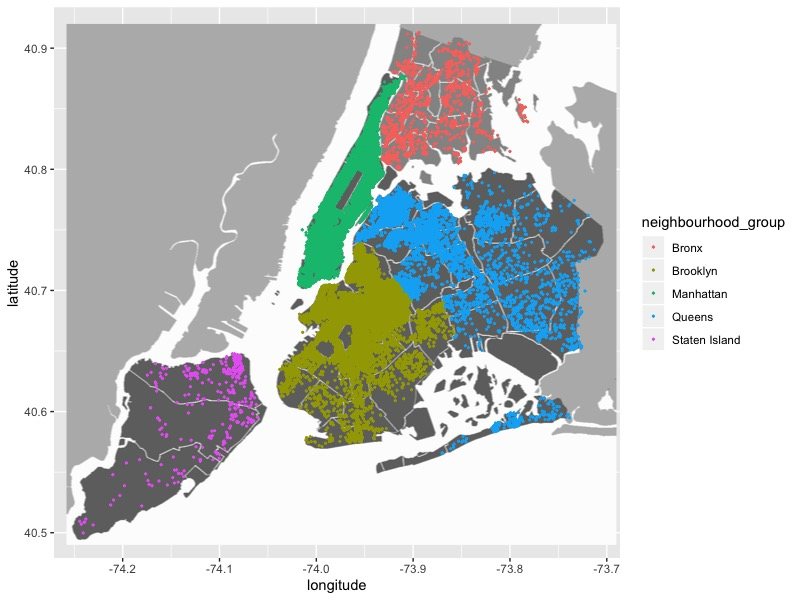
\includegraphics[scale=0.4]{Borough.jpeg}
\end{frame}




\begin{frame}
    \frametitle{EDA-price}
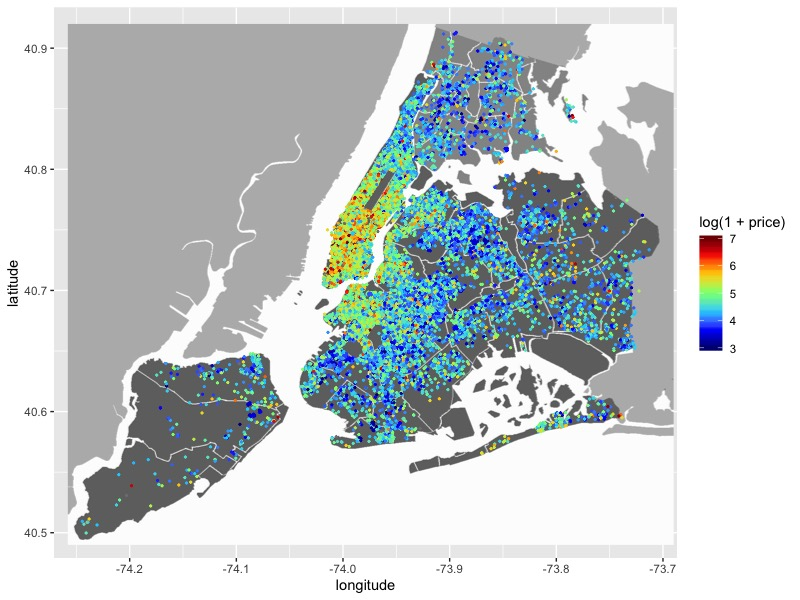
\includegraphics[scale=0.4]{price.jpeg}
\end{frame}

\begin{frame}
    \frametitle{EDA-Traffic}
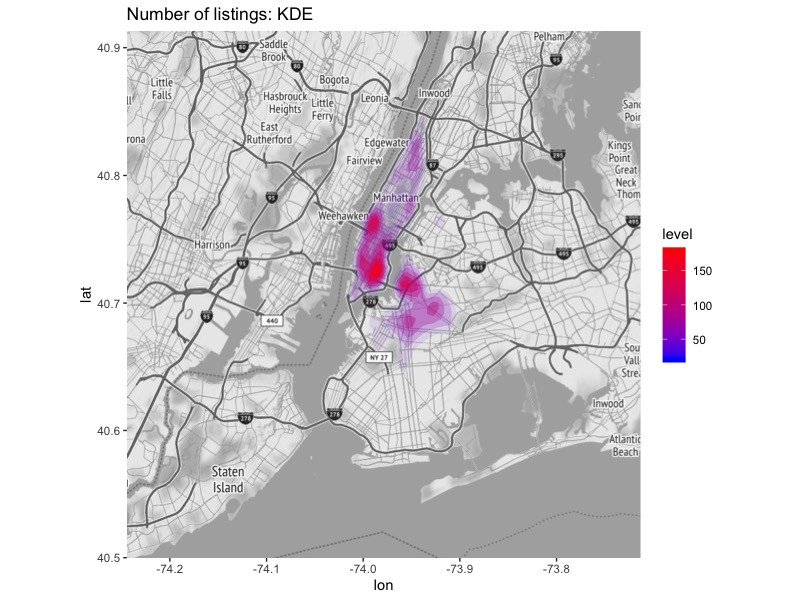
\includegraphics[scale=0.4]{KDE.jpeg}
\end{frame}


\begin{frame}
\frametitle{Model}
\begin{itemize}
	\item Multilevel Conditional Autoregressive (CAR) Model
$$ \begin{aligned}
 	Y_{kj}|\mu_{kj} \sim f(y_{kj}|\mu_{kj}, \nu^2), \ \ \ &k= \text{neighbourhood}
=1,...,K\\
  &j=\text{listings}=1,...,m_k \end{aligned}$$
$$g(\mu_{kj})=x_{kj}^T\beta + \psi_{kj}$$
$$\psi_{kj}=\phi_k + \zeta_{kj}$$
\item Priors
$$\beta \sim N(\mu_\beta, \Sigma_\beta)$$
$$\phi_k|\phi_{-k} \sim N\Big(\frac{\rho \sum_{l=1}^K w_{kl}\phi_j}{\rho \sum_{j=1}^K w_{kl}+1-\rho}, \frac{\tau^2}{\rho\sum_{j=1}^Kw_{kl}+1-\rho}\Big)$$
\item $w_{kl}$ denotes whether neighborhood $k$ and $l$ are adjacent.
\item $\rho$ denotes spatial dependence.
\end{itemize}
$$  $$
\end{frame}








\begin{frame}
\frametitle{Model}
\begin{itemize}\item Priors (Cont'd)

	$$\begin{aligned}
	&\zeta_{kj}\sim N(0, \sigma^2)\\
	&\tau^2, \sigma^2\sim \text{Inv-Gamma} (a,b)\\
	&\rho \sim \text{Uniform(0,1)}
\end{aligned}$$

	\item $x_{kj}$ include room\_type, neighbourhood\_group, availability\_365, log(1+reviews\_per\_month), minimum\_nights, etc.
	\item  $\psi_{kj}=\phi_k + \zeta_{kj}$ includes both spatial information and individual random effect. 
\end{itemize}

\end{frame}




\begin{frame}
\frametitle{Further process the data}
\begin{itemize}
	\item No data for exactly 217 neighbourhoods.
	\item Relocate neighbourhoods according to formal NYC shapefile data (195 neighbourhoods).
	\item 191 neighbourhoods have airbnb listings.
	\item Obtain adjacency matrix $W=(w_{kl})$

\end{itemize}
	
\end{frame}

\begin{frame}
\frametitle{Neighbourhood Effect on log(price)}
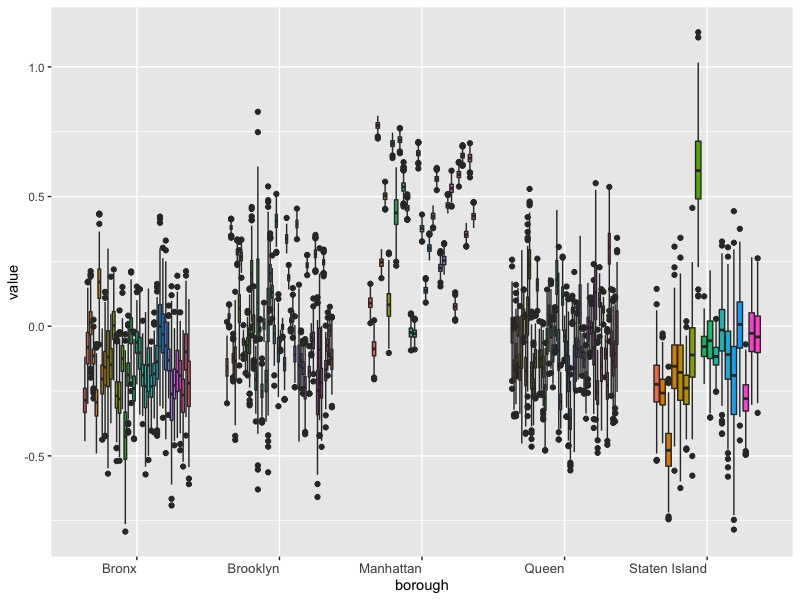
\includegraphics[scale=0.4]{CARBayes2.jpeg}

\end{frame}


\begin{frame}
\frametitle{Model Summary}
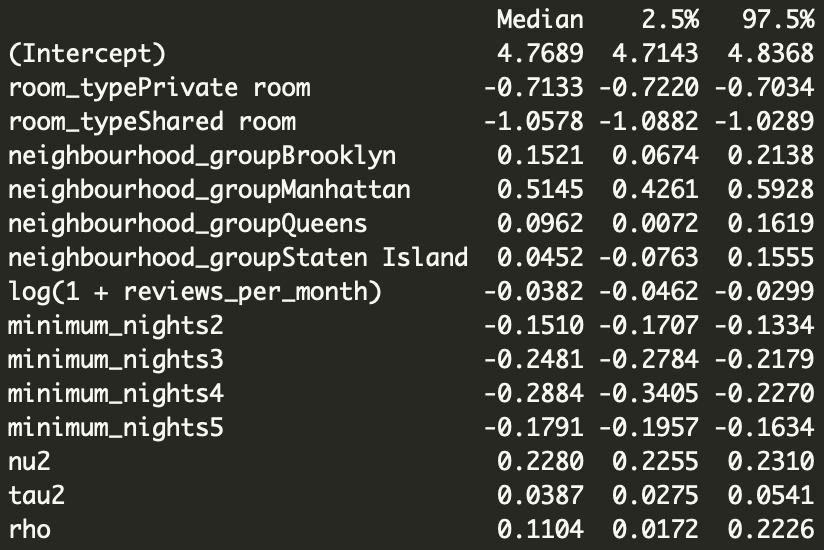
\includegraphics[scale=0.75]{summary.png}
\end{frame}





\begin{frame}
	\frametitle{Preliminary conclusion}
	\begin{itemize}
		\item Manhattan has highest prices, Bronx the lowest.
		\item Midtown South in Manhattan has the highest price.
		\item Entire room $>$ Private room $>$ Shared room
		\item Higher minimum\_nights leads to lower price. 
	\end{itemize}
\end{frame}








\begin{frame}
\frametitle{Discussion}
\begin{itemize}
	\item Include last\_review: spatial temporal model.
	\item Nonlinear model: spline regression for $x_{kj}$.
	\item More spatial information: longitude \& latitude
\end{itemize}
	
\end{frame}






\end{document}
